%==============================================================

\chapter{Big Data Framework Spark}\label{bds1}

After accumulating the data and presenting various methods to extract and process the different audio features, the following chapters describe the data analysis and computation of the similarities with Apache Spark \cite{spark}. Chapter \ref{bds1} deals with the implementation of the various similarity measurements while chapter \ref{bds2} deals with the handling of larger amounts of data, runtime analysis and the combination of multiple similarity measurements. 

\section{Apache Hadoop and Spark} 

First of all a small introduction to Big Data processing with Spark is given.
With the ever growing availability of huge amounts of high dimensional data the need for toolkits and efficient algorithms to handle these grew as well over the past years. Map-Reduce as a 

\subsection{Hadoop and Map Reduce}

\subsection{Spark and RDDs}

\subsection{Spark DataFrame}

\subsection{lazy evaluation}

\subsection{min and max value aggregation}

\textit{\textbf{Why? Scaling of distances between 0 to 1 interval to combine different distances\\}}

\FloatBarrier
\begin{figure}[htbp]
	\centering
	\framebox{\parbox{1\textwidth}{
			\begin{subfigure}{.495\textwidth}
				\centering
				\includegraphics[scale=0.22]{Images/Spark/separate.png}
				\caption{Separate DataFrames}
				\label{sc3}
			\end{subfigure}%
			
			\begin{subfigure}{.495\textwidth}
				\centering
				\includegraphics[scale=0.22]{Images/Spark/df_merged.png}
				\caption{Single DataFrames, multiple collects}
				\label{sc4}
			\end{subfigure}% 	
			
			\begin{subfigure}{.495\textwidth}
				\centering
				\includegraphics[scale=0.22]{Images/Spark/speed_uo.png}
				\caption{Single DataFrames, single collects}
				\label{sc5}
			\end{subfigure}% 		
	}}
	\caption{Spark DF implementations, single node, 1517 artists}
	\label{fig:spark2}
\end{figure}
\FloatBarrier


\section{Data locality and parallelization}

\noindent\textit{\textbf{high data locality, full parallelizable, very low replication rate\\}}
\noindent\textit{\textbf{insert data locality scheme here\\}}

\section{Combining different measurements}

\noindent\textit{\textbf{weighted arithmetic mean of different distance measurements\\}}

\begin{equation} \label{eq:distance}
dist = \frac{\sum_{m = 0}^{M - 1}{w_m \cdot d_m}}{\sum_{m = 0}^{M - 1}{w_m}}
\end{equation}

\noindent\textit{\textbf{statistic prescaling to have mean = 0.5 and variance 0.5?\\}}


\section{Data aggregation}

To work with the features a few transformations have to be done first. 

\begin{pythonCode}
song = "music/TURCA1.wav"
chroma = sc.textFile("features/out[0-9]*.notes")
chroma = chroma.map(lambda x: x.split(';'))
chroma = chroma.map(lambda x: (x[0], x[1], x[2], x[3].replace("10",'K').replace("11",'L').replace("0",'A').replace("1",'B').replace("2",'C').replace("3",'D').replace("4",'E').replace("5",'F').replace("6",'G').replace("7",'H').replace("8",'I').replace("9",'J')))
chroma = chroma.map(lambda x: (x[0], x[1], x[2], x[3].replace(',','').replace(' ','')))
df = spark.createDataFrame(chroma, ["id", "key", "scale", "notes"])
\end{pythonCode}

\noindent\textbf{\textit{Explain Single DataFrame vs multiple DataFrames}}

\section{Euclidean Distance}

\begin{pythonCode}
from scipy.spatial import distance
#...
distance_udf = F.udf(lambda x: float(distance.euclidean(x, comparator_value)), FloatType())
result = df_vec.withColumn('distances', distance_udf(F.col('features')))
result = result.select("id", "distances").orderBy('distances', ascending=True)
result = result.rdd.flatMap(list).collect()
\end{pythonCode}

\noindent\textit{\textbf{Explain usage of user defined function udf\\}}
\ \\
\noindent\textit{\textbf{Used with BH, RH, BP AND MFCC\\}}
\ \\
\noindent\textit{\textbf{super versatile AND very fast\\}}
\ \\
\noindent\textit{\textbf{insert analysis of performance\\}}

\section{Bucketed Random Projection}

\begin{pythonCode}
from pyspark.ml.feature import BucketedRandomProjectionLSH
#...
brp = BucketedRandomProjectionLSH(inputCol="features", outputCol="hashes", seed=12345, bucketLength=1.0)
model = brp.fit(df_vec)
comparator_value = Vectors.dense(comparator[0])
result = model.approxNearestNeighbors(df_vec, comparator_value, df_vec.count()).collect()
rf = spark.createDataFrame(result)
result = rf.select("id", "distCol").rdd.flatMap(list).collect()
\end{pythonCode}

\noindent\textit{\textbf{Usable as a substitute for euclidean UDF\\}}
\ \\
\noindent\textit{\textbf{Is it faster than the UDF tho? - performance test\\}}

\section{Cross-correlation}

\FloatBarrier
\begin{figure}[htbp]
	\centering
	\framebox{\parbox{1\textwidth}{
			\begin{subfigure}{.495\textwidth}
				\centering
				\includegraphics[scale=0.22]{Images/Spark/df_slow_chroma.png}
				\caption{Chroma multiple agg}
				\label{chr2}
			\end{subfigure}%
			
			\begin{subfigure}{.495\textwidth}
				\centering
				\includegraphics[scale=0.22]{Images/Spark/df_speed_chroma.png}
				\caption{Chroma single agg}
				\label{chr1}
			\end{subfigure}% 	
			
			\begin{subfigure}{.495\textwidth}
				\centering
				\includegraphics[scale=0.22]{Images/Spark/toPandasDag.png}
				\caption{DAG toPandas}
				\label{chr3}
			\end{subfigure}% 		
	}}
	\caption{Chroma on 11500 songs, single node}
	\label{fig:chroma}
\end{figure}
\FloatBarrier


\textit{\textbf{2 Versions explained - with additional key shift and without}}
\begin{pythonCode}
def cross_correlate(chroma1, chroma2):
    corr = sp.signal.correlate2d(chroma1, chroma2, mode='full')
    #transposed_chroma = transposed_chroma / (min(length1, length2))
    index = np.where(transposed_chroma == np.amax(transposed_chroma))
    index = int(index[0])
    mean_line = transposed_chroma[index]
    sos = sp.signal.butter(1, 0.1, 'high', analog=False, output='sos')
    mean_line = sp.signal.sosfilt(sos, mean_line)
    return np.max(mean_line)
#...
distance_udf = F.udf(lambda x: float(cross_correlate(x, comparator_value)), DoubleType())
result = df_vec.withColumn('distances', distance_udf(F.col('chroma')))
result = result.select("id", "distances").orderBy('distances', ascending=False)
result = result.rdd.flatMap(list).collect()
\end{pythonCode}

\noindent\textbf{\textit{Memory intense - had to alter spark-defaults.conf\\}}
\textit{spark.driver.memory             6g\\
spark.executor.memory           2g\\
}
\noindent\textbf{\textit{Insert graphics of calculation time with and without correlation\\}}
\ \\
\noindent\textbf{\textit{Differences in the results to the original paper can be explained with the different underlying beat tracking, different filter parameters and a few improvements that are left out as mentioned in \ref{chromafeat}}\cite{cover802}}

\section{Kullback-Leibler Divergence}

\begin{pythonCode}
def symmetric_kullback_leibler(vec1, vec2):
	#preprocessing: splitting vec1 and vec2 into mean1, mean2, cov1 and cov2
    d = 13
    div = 0.25 * (np.trace(cov1 * np.linalg.inv(cov2)) + np.trace(cov2 * np.linalg.inv(cov1)) + np.trace( (np.linalg.inv(cov1) + np.linalg.inv(cov2)) * (mean1 - mean2)**2) - 2*d)
    return div
distance_udf = F.udf(lambda x: float(symmetric_kullback_leibler(x, comparator_value)), DoubleType())
result = df_vec.withColumn('distances', distance_udf(F.col('features')))
result = result.select("id", "distances").orderBy('distances', ascending=True)
result = result.rdd.flatMap(list).collect()
\end{pythonCode}

\noindent\textbf{\textit{Differences in the results to the original musly tool can be explained due to the choice of only 13 MFCC bands in this thesis compared to the 25 bands in musly}\cite{musly1}}

\section{Jensen-Shannon Divergence}

\begin{pythonCode}
def jensen_shannon(vec1, vec2):
	#preprocessing: splitting vec1 and vec2 into mean1, mean2, cov1 and cov2
    mean_m = 0.5 * (mean1 + mean2)
    cov_m = 0.5 * (cov1 + mean1 * np.transpose(mean1)) + 0.5 * (cov2 + mean2 * np.transpose(mean2)) - (mean_m * np.transpose(mean_m))
    div = 0.5 * np.log(np.linalg.det(cov_m)) - 0.25 * np.log(np.linalg.det(cov1)) - 0.25 * np.log(np.linalg.det(cov2))  
    if np.isnan(div):
        div = np.inf
    return div
distance_udf = F.udf(lambda x: float(jensen_shannon(x, comparator_value)), DoubleType())
result = df_vec.withColumn('distances', distance_udf(F.col('features')))
result = result.select("id", "distances").orderBy('distances', ascending=True)
result = result.rdd.flatMap(list).collect()
\end{pythonCode}

\noindent\textbf{\textit{Problem mit den "skyrocketing determinanten" -> Lösung: cholesky zerlegung, geht nicht - nicht positiv definit, Lösung 2 nutzen von SKL aber noch rechenintensiver!}\cite[p.45]{schnitzer1}}

\section{Levenshtein distance}

\begin{pythonCode}
def get_neighbors_notes(song):
    filterDF = df.filter(df.id == song)
    filterDF.first()
    comparator_value = filterDF.collect()[0][3] 
    print comparator_value
    df_merged = df.withColumn("compare", lit(comparator_value))
    df_levenshtein = df_merged.withColumn("word1_word2_levenshtein", levenshtein(col("notes"), col("compare")))
    df_levenshtein.sort(col("word1_word2_levenshtein").asc()).show()
\end{pythonCode}

\section{performance}

\subsection{Performance Comparison of RDD vs DataFrame}

\FloatBarrier
\begin{figure}[htbp]
	\centering
	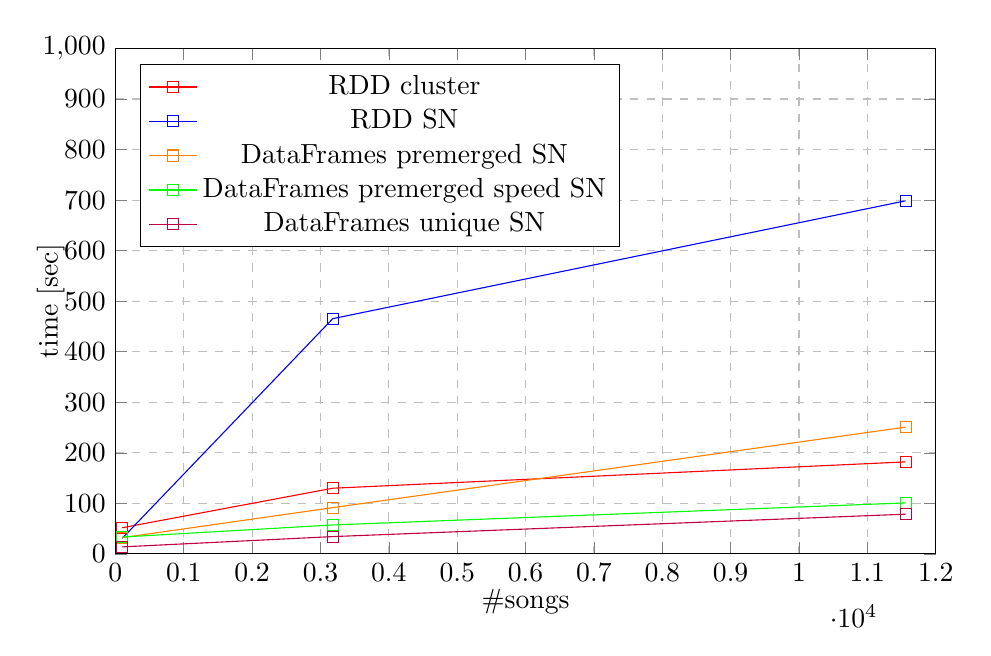
\begin{tikzpicture}
	\centering
	\begin{axis}[
	    %title={Performance of various toolkits},
		x label style={at={(axis description cs:0.5,-0.05)},anchor=north},
		y label style={at={(axis description cs:-0.05,.5)},rotate=0,anchor=south},
	    xlabel={\#songs},
	    ylabel={time [sec]},
	    xmin=0, xmax=12000,
	    ymin=0, ymax=1000,
	    xtick={0,1000,2000,3000,4000,5000,6000,7000,8000,9000,10000,11000,12000},
	    ytick={0,100,200,300,400,500,600,700,800,900,1000},
	    legend pos=north west,
	    ymajorgrids=true,
	    grid style=dashed,
	    height=8cm,
	    width=12cm,
	    grid=major,
	]
	\addplot[
		color=red,
		mark=square,
		]
		coordinates {
	    (100,51.736)(3180,129.940)(11560,182.035)
		};
		\addlegendentry{RDD cluster}
	\addplot[
	    color=blue,
	    mark=square,
	    ]
	    coordinates {
	    (100,30.770)(3180,465.445)(11560,698.657)
	    };
	    \addlegendentry{RDD SN}
	\addplot[
	    color=orange,
	    mark=square,
	    ]
	    coordinates {
	    (100,32.087)(3180,91.477)(11560,250.854)
	    };
	    \addlegendentry{DataFrames premerged SN}
	  
	\addplot[
	    color=green,
	    mark=square,
	    ]
	    coordinates {
	    (100,33.351)(3180,57.230)(11560,100.884)
	    };
	    \addlegendentry{DataFrames premerged speed SN}

	\addplot[
	    color=purple,
	    mark=square,
	    ]
	    coordinates {
	    (100,13.874)(3180,34.232)(11560,78.566)
	    };
	    \addlegendentry{DataFrames unique SN}	    
	\end{axis}
	\end{tikzpicture}
	\caption{Performance of various spark algorithms (MFCC Euc, Notes, RP)}
	\label{perfspark}
\end{figure}
\FloatBarrier

\section{feature separation quality}

\textit{\textbf{Which features are useful, which not (looking at you rhythm histogram)\\}}
\\

\textbf{\textit{\underline{correlation of features\\}}} 
\begin{figure}[htbp]
	\centering
	\framebox{\parbox{1\textwidth}{ 			
			\begin{subfigure}{.495\textwidth}
				\centering    
				\includegraphics[scale=0.35]{Images/SparkFeat/correlation1517_95.png}
				\caption{95 songs from 19 genres, 1517 artists}
				\label{cor1}
			\end{subfigure}		
			\begin{subfigure}{.495\textwidth}
				\centering     
				\includegraphics[scale=0.35]{Images/SparkFeat/correlation10.png}
				\caption{10 songs from 4 genres, full ds}
				\label{cor2}
			\end{subfigure}%		
	}}
	\caption{correlation of features}
	\label{fig:corr}
\end{figure}


\textbf{\textit{\underline{correlation of features\\}}} 
\begin{figure}[htbp]
	\centering
	\framebox{\parbox{1\textwidth}{ 			
			\includegraphics[scale=0.33]{Images/SparkFeat/corr_95_1517.png}	
	}}
	\caption{correlation 95 songs, 19 genres (5 each), 1517 artists}
	\label{fig:corr2}
\end{figure}

\textbf{\textit{\underline{distances from classical song out of 1517 artists dataset\\}}} 
\begin{figure}[htbp]
	\centering
	\framebox{\parbox{1\textwidth}{ 			
			\begin{subfigure}{.495\textwidth}
				\centering    
				\includegraphics[scale=0.3]{Images/SparkFeat/BH_BPM.png}
				\caption{Beat Histogram vs BPM}
				\label{fs1}
			\end{subfigure}		
			\begin{subfigure}{.495\textwidth}
				\centering     
				\includegraphics[scale=0.5]{Images/SparkFeat/MFCC_Eucl.png}
				\caption{MFCC Euclidean}
				\label{fs2}
			\end{subfigure}%	
			
			\begin{subfigure}{.495\textwidth}
				\centering    
				\includegraphics[scale=0.5]{Images/SparkFeat/BH_RP.png}
				\caption{Beat Histogram vs Rhythm Patterns}
				\label{fs3}
			\end{subfigure}
			\begin{subfigure}{.495\textwidth}
				\centering     
				\includegraphics[scale=0.5]{Images/SparkFeat/Cross-Corr_Levenshtein.png}
				\caption{Cross-correlation vs Levenshtein}
				\label{fs4}
			\end{subfigure}%		
	}}
	\caption{genre recall 100 songs}
	\label{fig:featsep}
\end{figure}


\section{possible performance improvements}

\textit{\textbf{Pre- merge feature sets, broadcast comparator, descending importance pre-filtering\\}}
\\
\textit{\textbf{statistic normalization of similarities\\}}
\ \\
\textit{\textbf{Filter and refine after statistic normalization, drop all below mean\\}}
\ \\
\textit{\textbf{\underline{Is there a better way to cross-correlate???}\\}}
\ \\
\section{Other alternatives}

\subsection{Alternating Least Squares}

\subsection{TF-IDF weights}

\subsection{DIMSUM all-pairs similarity}